\chapter{Modellierung und Zustandsraumdarstellung des Doppelpendels}

Die Grundlage f�r die Simulation des inversen Doppelpendels bilden die dynamischen Bewegungsgleichungen. In diesem Kapitel wird auf die Herleitung der Gleichungen eingegangen. Des Weiteren wird auf die f�r die hier dargestellten Regelungskonzepte des inversen Doppelpendels notwendige Zustandsraumdarstellung erl�utert.  

\section{Dynamische Gleichungen}

Der Aufbau des inversen Doppelpendels kann \bild{skizze_dp} entnommen werden. Das System besteht aus einem Wagen und zwei miteinander verbundenen St�ben. Der Wagen ist auf einer Linearf�hrung verschiebbar 

\begin{figure}[!ht]
	\begin{center}
		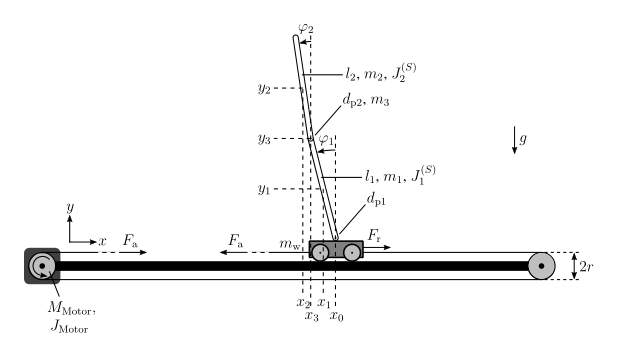
\includegraphics{skizze_dp}
		\caption{Aufbau des inversen Doppelpendels}
		\label{fig.skizze_dp}
	\end{center}
\end{figure}

%\begin{equation}
%sljdsjuhd = luhsdfiuhsf+ spidhfos
%\end{equation}

